\documentclass{thecours}
\let\mathspoint\textsf
\begin{document}
    \bigpart{Vocabulaire et notations}
    \subpart{Vocabulaire}
    \definition{angle}
    \vskip5pt\par\noindent{\bfseries Exemple :}\vskip5pt\par\noindent
    \begin{minipage}{.35\linewidth}
        \exported[scale=1.5, ]%
            <<%
        \begin{tikzpicture}[line width=1pt]
            \AnglexOy[
                right side len = 3,
                left side len = 3,
                angle = 45,
                color = \currentcolor%
                ]
        \end{tikzpicture}>>
    \end{minipage}\hspace{.01\linewidth}
    \begin{minipage}{.45\linewidth}
        Le sommet est le point \mathspoint{O}.\par\noindent
        Les côtés sont \mathspoint{[Ox)} et \mathspoint{[Oy)}.
    \end{minipage}\vskip10pt
    \subpart{Notations}
    \regle{notation_angle}\vskip5pt\par\noindent
    {\bfseries Exemple : } L'angle du premier exemple se note $\widehat{\mathspoint{xOy}}$.\vskip10pt
    \subpart{Nature des angles}
    \exported[scale=1.2, ]%
            <<%
    \begin{tikzpicture}[scale=.8]
        \AnglexOy[
        angle = 40,
        color=\currentcolor,
        right side len = 3,
        left side len = 2,
        left side pos = above left
        ]
        \draw[colored, dotted, line width=1.2pt](0,0)--(0,3);
    \end{tikzpicture}\hfill
    \begin{tikzpicture}[scale=.8]
        \AnglexOy[
        angle = 90,
        color=white,
        right side len = 2,
        left side len = 2,
        left side pos = above left
        ]
        \tkzMarkRightAngle[size=.5, colored](B,A,C)
        \draw[colored, dotted, line width=1.2pt](0,0)--(0,3);
    \end{tikzpicture}\hfill
    \begin{tikzpicture}[scale=.8]
        \AnglexOy[
        angle = 140,
        color=\currentcolor,
        right side len = 2,
        left side len = 2,
        left side pos = below left,
        angle size=.8
        ]
        \draw[colored, dotted, line width=1.2pt](0,0)--(0,3);
    \end{tikzpicture}\hfill
    \begin{tikzpicture}[scale=.8]
        \AnglexOy[
        angle = 180,
        color=\currentcolor,
        right side len = 1.5,
        left side len = 1.5,
        left side pos = below left,
        angle size=.5
        ]
        \draw[colored, dotted, line width=1.2pt](0,0)--(0,3);
    \end{tikzpicture}\hfill\par\noindent
    \toComplete{Angle aigu}\hfill \toComplete{Angle droit}\hfill \toComplete{Angle obtus}\hfill \toComplete{Angle plat}\hfill
    >>
    \bigpart{Mesurer un angle}
    \par\noindent\definition{mesure_d_un_angle}
    {\par\noindent\centering
        \pdf[scale=.7]{6eme_Indigo_206_2}
    \centering}
    \par\noindent
    \definition{rapporteur}
    \exported[scale=1.2, ]%
            <<%
    \begin{tblr}{colspec={Q[c,m]Q[c,m]Q[c,m]}}
        
\begin{tikzpicture}[scale=1]
            \Angle[
            right side len = 3,
            left side len = 3,
            angle = 90,
            color = white
            ]
            \tkzMarkRightAngle[size=.5, colored](B,A,C)
            \toComplete{\tkzLabelAngle[pos=1.5](B,A,C){{$\mathbf{90}^\circ$}}}
        \end{tikzpicture}&
        \begin{tikzpicture}[scale=1]
            \Angle[
            right side len = 3,
            left side len = 3,
            angle = 70,
            color = \currentcolor
            ]
            \toComplete{\tkzLabelAngle[pos=1.5](B,A,C){{$\mathbf{70}^\circ$}}}
        \end{tikzpicture}&
        \begin{tikzpicture}[scale=1]
            \Angle[
            right side len = 3,
            left side len = 3,
            angle = 115,
            color = \currentcolor
            ]
            \toComplete{\tkzLabelAngle[pos=1.5](B,A,C){{$\mathbf{115}^\circ$}}}
        \end{tikzpicture}\\
        \toComplete{Angle droit}&\toComplete{Angle aigu}&\toComplete{Angle obtus}
    \end{tblr}
    >>\par
    \newpage
    \bigpart{Tracer un angle}
    \exported[scale=1.2, ]%
    <<\par\noindent\begingroup\centering
    \pdf[scale=.85]{6eme_Indigo_208_3}
    \centering\endgroup>>
    \vskip5pt\par\noindent{\bfseries Exemple :}
    \begin{enumerate}[label=\alph*)]
        \item Tracer un angle $\widehat{\mathspoint{XZY}}$ de mesure $70^\circ$.
        \vskip15pt\par\noindent\hskip50pt
        \begin{tikzpicture}[scale=.6]
            \AngleAOB[
            sommet name = Z,
            right side name = X,
            left side name = Y,
            right side len = 3,
            left side len = 3,
            angle = 70,
            color = \currentcolor
            ]
            \tkzLabelAngle[pos=1.5](B,A,C){{$\mathbf{70}^\circ$}}
        \end{tikzpicture}\hfill\vskip15pt
        \item Tracer un angle $\widehat{\mathspoint{rOs}}$ de mesure $155^\circ$.
        \vskip15pt\par\noindent\hskip50pt
        \begin{tikzpicture}[scale=.6]
            \AnglexOy[
            sommet name = Z,
            right side name = r,
            left side name = s,
            right side len = 3,
            left side len = 3,
            left side pos = below left,
            angle = 155,
            color = \currentcolor
            ]
            \tkzLabelAngle[pos=1.5](B,A,C){{$\mathbf{155}^\circ$}}
        \end{tikzpicture}\hfill\vskip15pt
    \end{enumerate}
\end{document}